\chapter{Scientific Background\label{cha:chapter2}}

This chapter reviews the material Chapter~\ref{cha:chapter4} builds on: distribution-aware dataset search and the Fainder index (§\ref{sec:bg:dataset-search}), the hardware and systems-programming material relevant to the four ceilings (§\ref{sec:bg:hardware}), and a primer on what it means for two hardware-conscious optimisations to compose (§\ref{sec:bg:composability}).
A reader comfortable with these topics can jump to Chapter~\ref{cha:chapter3}.

\section{Distribution-Aware Dataset Search\label{sec:bg:dataset-search}}

\subsection{Data Discovery and Distribution-Aware Search}

Open data lakes and data collected in corporate catalogs are usually in the range of having millions of columns. Data scientists with a particular statistical profile of data in mind (for example, columns with a median between $50$ and $100$, or data in which the 90th percentile has a certain cutoff) would usually need to scan every file. \emph{Distribution-aware dataset search}~\cite{behme_2024} is the class of search problems whose predicates concern the distribution of column values, rather than schema or keywords.

How such predicates are answered depends on what is accessible. For federated and privacy-sensitive data, the raw values are often not readable at all; the only available evidence is statistical metadata such as per-column histograms, computed before access is restricted~\cite{behme_2024}. This thesis targets that setting, and within it the percentile-predicate instance of distribution-aware search: given a collection of histograms $\mathcal{H} = \{h_1, \ldots, h_n\}$ summarising individual columns, a query $\langle p, \bowtie, \tau \rangle$ must return every histogram $h$ for which the $p$-th percentile of $h$ satisfies $h[p] \bowtie \tau$, without ever touching the underlying rows.

\subsection{Fainder Index}

Fainder~\cite{behme_2024} is a three-phase index that exists for this type of query.

\textbf{Index construction.} In this phase, we group $n$ histograms into $k$ clusters by using K-means on the histogram vectors. In each cluster, we align the histograms onto a shared bin grid. Fainder makes use of two alignment strategies: \emph{rebinning}, which projects each histogram onto a fixed bin count, which is compact and fast, with a small alignment error near bin boundaries and \emph{conversion}, which produces two index variants per cluster (a rebinned variant plus a higher-accuracy converted variant), at $\approx 2\times$ the memory cost and a $10$--$15\%$ slower query. In this thesis we use rebinning throughout the entire work, since the accuracy delta stays the same throughout all of our findings.

\textbf{Index structure.} \emph{FainderIndex} is a Union of all \emph{SubIndex}'s. Each cluster $c$ has a SubIndex that stores the cumulative density values of all histograms in $c$ at each bin boundary $b$. The cumulative density values are stored in a sorted array, along with the matching histogram identifiers. 

\textbf{Query execution.} To execute a query $\langle p, \bowtie, \tau \rangle$, the engine traverses through each cluster, where it searches the shared bin grid via binary search in order to find the bin $b^*$ that corresponds to the reference value $\tau$. Then, it performs another (binary) search on the cumulative density array at boundary $b^*$ to collect the saved histogram IDs that follow the percentile predicate. The $\cup$ across all clusters is the final answer.

The query phase can be thought of as a sequence of binary searches, one per cluster. Because each cluster's search is a chain of dependent loads, this thesis focuses on cache- and memory-hierarchy effects rather than SIMD throughput on streaming scans.

\section{Hardware-Conscious System Design\label{sec:bg:hardware}}

In this section we cover the hardware and systems-programming background that Chapter~\ref{cha:chapter4} builds on. The goal of this section is to be a reference point for each of the ceilings introduced in Chapter~\ref{cha:chapter1}. This also references the systems programming techniques used in the Rust implementation of Fainder, which is described in Chapter~\ref{cha:chapter3}.


\subsection{Modern Superscalar CPU Architecture\label{sec:bg:cpu}}

Modern server CPUs are out-of-order superscalar processors. The ancestor of these processors is Tomasulo's 1967 dynamic-scheduling algorithm~\cite{tomasulo_1967}. In the CPU, each core fetches and decodes instructions in the front-end and dispatches them to a reorder buffer (ROB). ROB depth scales with generation, from $\sim\!200$ on Skylake to $512$ entries on Golden Cove (the microarchitecture of the Sapphire Rapids Xeon 8468H used in this thesis). Each core has several execution ports that can perform multiple operations per cycle~\cite{hennessy_2017,fog_optimization}. Retirement width is also generation-dependent (4-wide on Skylake, up to 8-wide on Golden Cove). The IPC ceiling on this platform is therefore not the four-wide figure typical of older cores~\cite{intel_optimization_manual}.

Instructions per cycle (IPC) is $\frac{\text{retired instructions}}{\text{cycles}}$. If a program is scalar and serial, and never stalls, it can approach the retirement width of the core (four on Skylake-class, higher on Golden Cove). The three main stall categories that push IPC below the ceiling in practice are:

\begin{enumerate}
  \item \emph{Front-end stalls}: the instruction fetch mechanism can't keep up, which usually happens after a branch misprediction (Section~\ref{sec:bg:branch}).
  \item \emph{Back-end stalls}: the execution ports are fully utilised, either because there are not enough independent instructions to fill them or because a dependency chain serialises the work.
  \item \emph{Memory stalls}: a load waits for data. L1 hit takes $\sim\!4$--$5$ cycles, L2 hit $\sim\!12$--$15$, L3 hit roughly $40$. DRAM depends on locality, $\sim\!170$--$320$ cycles for a local (on-socket) DDR5 access at $2.1$--$3.8$\,GHz, and roughly twice that for a remote access over UPI (see §\ref{sec:bg:numa}).
\end{enumerate}

Work by Yasin~\cite{yasin_2014} breaks the stall cycles into these categories. An IPC near the retirement ceiling indicates compute-bound work with healthy instruction-level parallelism, an IPC of $\approx 1$ typically means the work is either heavily dependent or memory-bound.

If a cache miss stalls a load, the ROB can dispatch independent instructions to overlap the miss latency, modern CPUs rely on this to tolerate slow memory. The scenario where this cannot be used is when a load is \emph{dependent} on the one before it, so load $i+1$ cannot be issued until load $i$ completes. Binary search is the canonical example: each step reads \texttt{arr[mid]}, and the next \texttt{mid} depends on the current comparison result, which serialises the load chain and defeats out-of-order execution.

\subsection{Memory Hierarchy and Cache Efficiency\label{sec:bg:memory}\label{sec:sb:memhier}}

There are three layers of caches that sit between the core and DRAM, hierarchically:
\begin{itemize}
  \item \textbf{L1 cache} is the smallest and fastest, typically tens of KB per core. It has the lowest latency, around $4$--$5$ cycles for a hit.
  \item \textbf{L2 cache} is larger, typically a few MB per core. It has a higher latency, around $12$--$15$ cycles for a hit.
  \item \textbf{L3 cache} is the largest and slowest, typically tens of MB shared across cores on the same socket. It has a higher latency, around $40$ cycles for a hit.
\end{itemize}

Above all of these sits the DRAM~\cite{hennessy_2017,drepper_2007}. A cache line (which is essentially a block of memory that is transferred between the cache and DRAM) is typically $64$ bytes wide. Manegold et al. \ looked at cache-conscious analysis for database operators~\cite{manegold_2000}.

Figure~\ref{fig:mem_hierarchy_latency} demonstrates the access latencies of each level of the memory hierarchy on the platform used for this thesis. There are dotted vertical cutoffs that indicate the working-set size at which we involve the next, slower level of the hierarchy. The x axis is logarithmic, with the unit of nanoseconds, since we span six orders of magnitude from $\sim\!1$\,ns to $\sim\!5$\,ms. Due to the shift in order of magnitude, we can observe measurable wall-time changes when we shift a working set from L3 into DRAM, but any experiment that bottlenecks on disk-backed storage will be dominated by the disk latency, and the cache hierarchy will be largely irrelevant.

\begin{figure}[h]
\centering
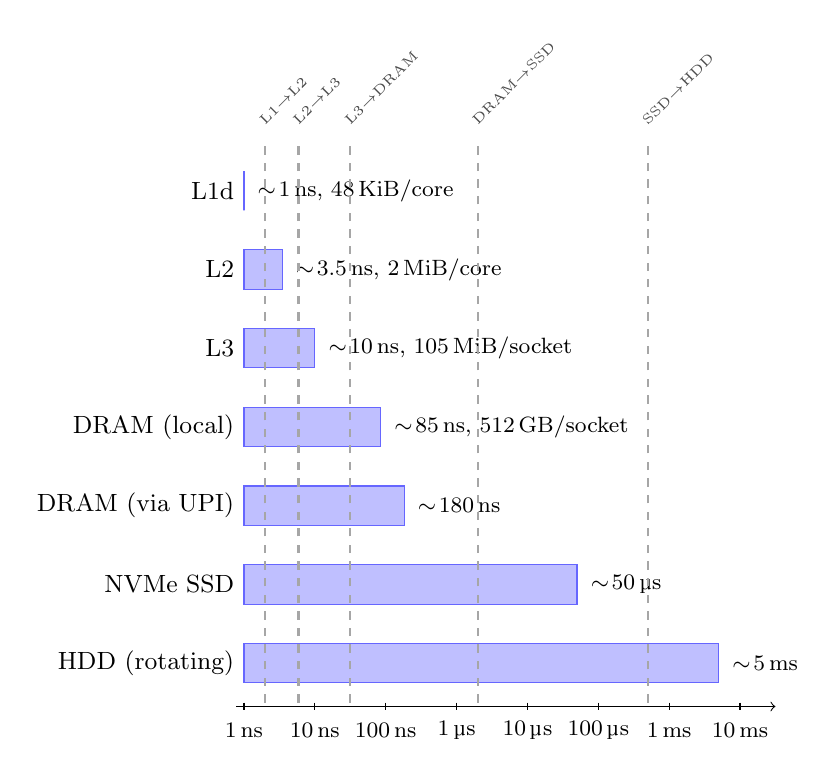
\begin{tikzpicture}[
    latbar/.style={rectangle, minimum height=5mm, anchor=west, fill=blue!25, draw=blue!60},
    cutoff/.style={dashed, gray!70, thick},
    ylabel/.style={anchor=east, font=\small},
    xlabel/.style={font=\footnotesize},
    valuelabel/.style={anchor=west, font=\footnotesize}
]
% Reference latencies: values in log10(latency in ns).
% L1d 1 ns (0.0), L2 3.5 ns (0.54), L3 10 ns (1.0), DRAM local 85 ns (1.93),
% DRAM remote (via UPI) 180 ns (2.26), NVMe SSD 50 us = 50000 ns (4.7), HDD 5 ms (6.7).
\pgfmathsetmacro{\xscale}{0.9}
\node[ylabel] at (0, 6) {L1d};
\draw[latbar] (0, 5.75) rectangle ({\xscale * 0.0}, 6.25);
\node[valuelabel] at ({\xscale * 0.0 + 0.05}, 6) {$\sim\!1$\,ns, 48\,KiB/core};

\node[ylabel] at (0, 5) {L2};
\draw[latbar] (0, 4.75) rectangle ({\xscale * 0.54}, 5.25);
\node[valuelabel] at ({\xscale * 0.54 + 0.05}, 5) {$\sim\!3.5$\,ns, 2\,MiB/core};

\node[ylabel] at (0, 4) {L3};
\draw[latbar] (0, 3.75) rectangle ({\xscale * 1.0}, 4.25);
\node[valuelabel] at ({\xscale * 1.0 + 0.05}, 4) {$\sim\!10$\,ns, 105\,MiB/socket};

\node[ylabel] at (0, 3) {DRAM (local)};
\draw[latbar] (0, 2.75) rectangle ({\xscale * 1.93}, 3.25);
\node[valuelabel] at ({\xscale * 1.93 + 0.05}, 3) {$\sim\!85$\,ns, 512\,GB/socket};

\node[ylabel] at (0, 2) {DRAM (via UPI)};
\draw[latbar] (0, 1.75) rectangle ({\xscale * 2.26}, 2.25);
\node[valuelabel] at ({\xscale * 2.26 + 0.05}, 2) {$\sim\!180$\,ns};

\node[ylabel] at (0, 1) {NVMe SSD};
\draw[latbar] (0, 0.75) rectangle ({\xscale * 4.7}, 1.25);
\node[valuelabel] at ({\xscale * 4.7 + 0.05}, 1) {$\sim\!50$\,\textmu s};

\node[ylabel] at (0, 0) {HDD (rotating)};
\draw[latbar] (0, -0.25) rectangle ({\xscale * 6.7}, 0.25);
\node[valuelabel] at ({\xscale * 6.7 + 0.05}, 0) {$\sim\!5$\,ms};

% Cutoffs — vertical dotted lines annotating boundary transitions.
% Labels rotated 45° with south-west anchor so they slant up-right from
% each cutoff line and do not overlap in the left-side cluster (L1->L2,
% L2->L3 are only ~0.4 units apart horizontally).
\draw[cutoff] ({\xscale * 0.3}, -0.5) -- ({\xscale * 0.3}, 6.6);
\node[font=\tiny, gray!60!black, anchor=south west, rotate=45] at ({\xscale * 0.3}, 6.65) {L1$\to$L2};
\draw[cutoff] ({\xscale * 0.77}, -0.5) -- ({\xscale * 0.77}, 6.6);
\node[font=\tiny, gray!60!black, anchor=south west, rotate=45] at ({\xscale * 0.77}, 6.65) {L2$\to$L3};
\draw[cutoff] ({\xscale * 1.5}, -0.5) -- ({\xscale * 1.5}, 6.6);
\node[font=\tiny, gray!60!black, anchor=south west, rotate=45] at ({\xscale * 1.5}, 6.65) {L3$\to$DRAM};
\draw[cutoff] ({\xscale * 3.3}, -0.5) -- ({\xscale * 3.3}, 6.6);
\node[font=\tiny, gray!60!black, anchor=south west, rotate=45] at ({\xscale * 3.3}, 6.65) {DRAM$\to$SSD};
\draw[cutoff] ({\xscale * 5.7}, -0.5) -- ({\xscale * 5.7}, 6.6);
\node[font=\tiny, gray!60!black, anchor=south west, rotate=45] at ({\xscale * 5.7}, 6.65) {SSD$\to$HDD};

% x-axis
\draw[->] (-0.1, -0.55) -- ({\xscale * 7.5}, -0.55);
\foreach \x/\l in {0/{1\,ns}, 1/{10\,ns}, 2/{100\,ns}, 3/{1\,\textmu s}, 4/{10\,\textmu s}, 5/{100\,\textmu s}, 6/{1\,ms}, 7/{10\,ms}} {
  \draw ({\xscale * \x}, -0.5) -- ({\xscale * \x}, -0.6);
  \node[xlabel] at ({\xscale * \x}, -0.85) {\l};
}
\end{tikzpicture}
\caption[Memory-hierarchy access latencies on the measurement platform.]{Access latencies along with the capacity of each level of the memory hierarchy on the Sapphire Rapids (Xeon 8468H) platform. X axis is logarithmic, with dotted lines along the Y axis indicating the working-set size at which the next slower level takes over (approximate transitioning zones, not exact cutoffs). The latencies illustrated are approximate values for warm access, not peak throughput. Exact numbers may vary depending on prefetcher state, memory controller queueing, and NUMA policy.}
\label{fig:mem_hierarchy_latency}
\end{figure}


Multiple prefetchers are attached to each core, they monitor access patterns and pull cache lines ahead of demand. L1 stride prefetchers catch sequential and constant-stride accesses (common in linear scans). L2 streamers catch coarser patterns. Neither can predict the data-dependent addresses of binary search, so binary search and other pointer-chasing or indirect-lookup workloads see little prefetcher help.

A core can hold multiple L1 misses in flight at once through Line-Fill Buffers (LFBs), their per-core count is $\sim\!10$ on Skylake and $\sim\!16$ on Golden Cove. Independent loads that all miss L1 perform round-trips to DRAM in parallel, which amortises the latency. A dependent load cannot benefit from this: the address of the next load is not known until the previous one is returned.

There is a fixed bytes-per-second budget for each DRAM channel. The Xeon 8468H used in this thesis has eight DDR5-4800 channels per socket, giving a per-socket peak of $\sim\!300$\,GB/s, and the two sockets together provide $\sim\!600$\,GB/s. When multiple cores stream data at once, that budget becomes contended and the effective per-core bandwidth drops. This differs from DRAM \emph{latency}, which is the round-trip time of one load: bandwidth only becomes binding when the aggregate traffic across all cores approaches the channel capacity.

The main hot path in Fainder is a binary search over a sorted column of cumulative density values. With an SoA layout, each cache line loaded contains only percentile values. With an AoS layout, half of every line is histogram-IDs that the search phase never reads. The pollution halves the values-per-line ratio. Chapter~\ref{cha:chapter4} shows this layout effect is measurable but small once larger ceilings dominate at scale.

\subsection{NUMA and the Cross-Socket Interconnect\label{sec:bg:numa}}

Servers with multiple sockets split their DRAM into per-socket \emph{NUMA nodes}~\cite{lameter_2013}. Each socket reaches its local node at normal DRAM latency, but reaches the other socket's node with an additional round-trip over Intel's Ultra-Path Interconnect (UPI) link between the two CPU packages. On the platform used in this thesis, \texttt{numactl -H} reports a NUMA distance of $10$ for local access and $21$ for cross-socket access, roughly a $2.1\times$ latency penalty on remote loads. The NUMA performance pathologies that appear in multicore workloads when allocations and threads end up on different nodes are catalogued by McCurdy and Vetter~\cite{mccurdy_2010}.

This thesis uses a two-socket platform with $96$ physical cores, and $48$ cores per socket. The default Linux scheduler does not constrain a thread to a single socket, so any thread count above $48$ will span both NUMA nodes out of necessity, which leads to cross-socket traffic. \texttt{numactl}'s \texttt{--membind} and \texttt{--cpunodebind} flags constrain a process to one node, which removes UPI traffic, but halves the core budget. 

For our fourth ceiling in Chapter~\ref{cha:chapter4} we use the cross-socket interconnect as our source of contention. Both UPI and on-socket DRAM fall under the label ``memory bandwidth'', but are binding under different conditions, and are measured differently. UPI has an empirical penalty that is distinguishable from the penalty for saturating local DRAM. The NUMA placement experiment of Chapter~\ref{cha:chapter4} separates the two.

\subsection{Structure of Arrays vs.\ Array of Structs\label{sec:sb:layouts}}

SoA vs AoS is a classical concern when designing data-oriented systems~\cite{manegold_2000}. Figure~\ref{fig:sb:soa_aos} illustrates the differences between them:

\begin{figure}[h]
\centering
\resizebox{0.95\linewidth}{!}{%
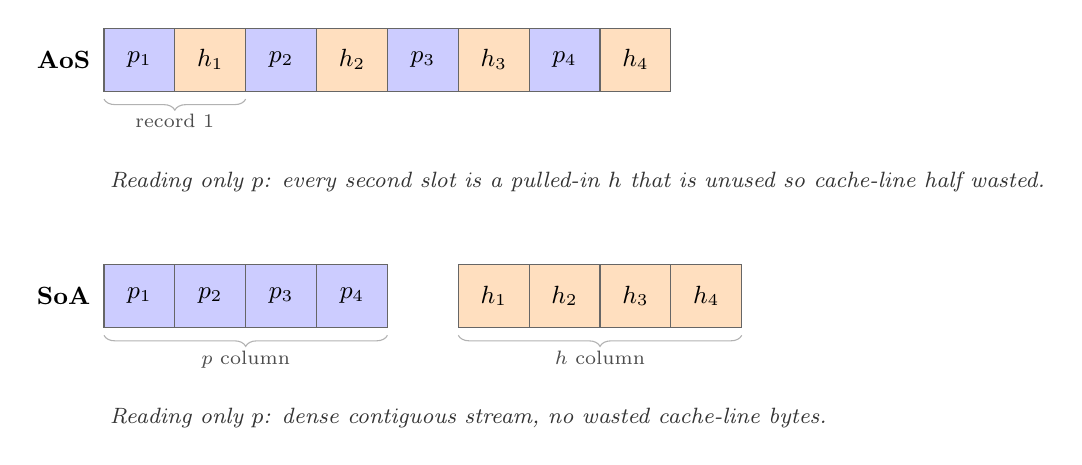
\begin{tikzpicture}[
    cell/.style={rectangle, draw=black!60, minimum width=9mm, minimum height=8mm, inner sep=0pt, font=\small},
    pcell/.style={cell, fill=blue!20},
    hcell/.style={cell, fill=orange!25},
    rowlbl/.style={font=\small\bfseries, anchor=east},
    notelbl/.style={font=\footnotesize, gray!40!black, anchor=west}
]

%  -- AoS row: interleaved (p_i, h_i) pairs  --
\node[rowlbl] at (0.5, 0) {AoS};
\foreach \i [count=\c] in {1,2,3,4} {
  \pgfmathsetmacro{\xp}{1.0 + (2*\c - 2) * 0.9}
  \pgfmathsetmacro{\xh}{1.0 + (2*\c - 1) * 0.9}
  \node[pcell] at (\xp, 0) {$p_\i$};
  \node[hcell] at (\xh, 0) {$h_\i$};
}
% Brace under the first record to make the grouping explicit
\draw[decorate, decoration={brace, amplitude=4pt, mirror}, gray!60]
  (0.55, -0.5) -- (2.35, -0.5)
  node[midway, below=2pt, font=\scriptsize, gray!60!black] {record 1};
\node[notelbl] at (0.5, -1.55) {\emph{Reading only $p$: every second slot is a pulled-in $h$ that is unused so cache-line half wasted.}};

%  -- SoA row: two separate contiguous arrays  --
\node[rowlbl] at (0.5, -3.0) {SoA};
\foreach \i [count=\c] in {1,2,3,4} {
  \pgfmathsetmacro{\xp}{1.0 + (\c - 1) * 0.9}
  \node[pcell] at (\xp, -3.0) {$p_\i$};
}
\foreach \i [count=\c] in {1,2,3,4} {
  \pgfmathsetmacro{\xh}{1.0 + (\c + 4) * 0.9}
  \node[hcell] at (\xh, -3.0) {$h_\i$};
}
% Braces under each column
\draw[decorate, decoration={brace, amplitude=4pt, mirror}, gray!60]
  (0.55, -3.5) -- (4.15, -3.5)
  node[midway, below=2pt, font=\scriptsize, gray!60!black] {$p$ column};
\draw[decorate, decoration={brace, amplitude=4pt, mirror}, gray!60]
  (5.05, -3.5) -- (8.65, -3.5)
  node[midway, below=2pt, font=\scriptsize, gray!60!black] {$h$ column};
\node[notelbl] at (0.5, -4.55) {\emph{Reading only $p$: dense contiguous stream, no wasted cache-line bytes.}};

\end{tikzpicture}%
}
\caption[AoS vs.\ SoA memory layout.]{AoS interleaves fields per record and SoA stores each field in its own contiguous array. For Fainder's access pattern (which touches only the percentile-value column ($p$) on every comparison), SoA halves the cache-line footprint by avoiding the unused hist-id ($h$) lanes.}
\label{fig:sb:soa_aos}
\end{figure}

SoA wins on cache utilisation when the access pattern is field-specific. For Fainder, only the percentile-value field is read during the search, and the histogram-ID is needed after the matching range has been located. SoA has about double the useful values per cache line. Chapter~\ref{cha:chapter4} quantifies this effect and shows it is regime-conditional: the advantage fades once memory-traffic pressure becomes the limiting ceiling at high thread counts.

\subsection{Eytzinger BFS Layout\label{sec:bg:eytzinger}}

During binary search, sorted arrays are accessed in a pseudo-random pattern, which is bad for cache locality. There are unpredictable strides that make the hardware prefetcher ineffective, and each access hits a new cache line. The \emph{Eytzinger BFS} (breadth-first) layout reorders a sorted array, such that the binary search tree is stored breadth-first. It stores the root at index~$0$, its children at $1$ and $2$, their children at $3\ldots 6$, and so on~\cite{khuong_morin_2017}. We can store the first four levels of that tree in a single 64-byte cache line, that means that the first four bisections of an array cost one line load, instead of four. The L1 stride prefetcher can help with subsequent levels, since they access consecutive positions $8, 9, 10, \ldots$ instead of scattered, random ones. Cache-oblivious analysis of layouts of this kind is attributed to research by Brodal and Fagerberg~\cite{brodal_fagerberg_2006}.

For searches of length $n$, this layout replaces $\log_2 n$ dependent-load stalls at pseudo-random offsets with a shorter sequence of loads at predictable stride, it also adds a bit-reversal permutation to convert the final BFS index back to the sorted-position index. This technique accelerates search when the cache is cold (when the searched array is not already in L1), at the cost of a small memory overhead. Benchmarks by Khuong and Morin~\cite{khuong_morin_2017} show wins for Eytzinger at large $n$ cold-cache searches, and small losses at small $n$ where the binary search already fits in L1 after a miss. In Fainder's per-cluster columns, Eytzinger's cache-cold advantage largely disappears since the columns are L1-resident after the first cluster access in a query batch. An early campaign in this thesis included a Cargo-gated Eytzinger variant, but the feature was dropped from the final integrated build described in Chapter~\ref{cha:chapter3}.

\begin{figure}[h]
\centering
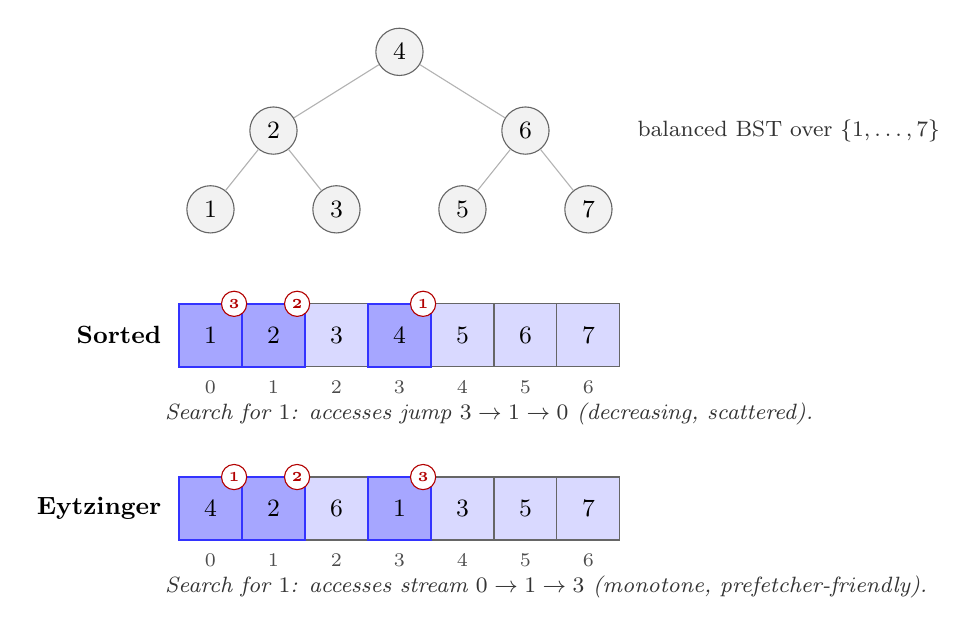
\begin{tikzpicture}[
    treenode/.style={circle, draw=black!60, fill=gray!10, minimum size=6mm, inner sep=0pt, font=\small},
    cell/.style={rectangle, draw=black!60, minimum width=8mm, minimum height=8mm, inner sep=0pt, font=\small},
    hcell/.style={cell, fill=blue!15},
    icell/.style={cell, fill=blue!35, draw=blue!80, thick},
    rowlbl/.style={font=\small\bfseries, anchor=east},
    idxlbl/.style={font=\scriptsize, gray!60!black, anchor=north},
    notelbl/.style={font=\footnotesize, gray!40!black, anchor=west},
    badge/.style={circle, draw=red!70!black, fill=white, font=\tiny\bfseries, text=red!70!black, inner sep=0.3pt, minimum size=3.2mm}
]

%  -- Balanced BST over {1,...,7}  --
\node[treenode] (root) at (3.6, 2.6) {4};
\node[treenode] (n2)   at (2.0, 1.6) {2};
\node[treenode] (n6)   at (5.2, 1.6) {6};
\node[treenode] (n1)   at (1.2, 0.6) {1};
\node[treenode] (n3)   at (2.8, 0.6) {3};
\node[treenode] (n5)   at (4.4, 0.6) {5};
\node[treenode] (n7)   at (6.0, 0.6) {7};
\draw[gray!60] (root) -- (n2);
\draw[gray!60] (root) -- (n6);
\draw[gray!60] (n2)   -- (n1);
\draw[gray!60] (n2)   -- (n3);
\draw[gray!60] (n6)   -- (n5);
\draw[gray!60] (n6)   -- (n7);
\node[notelbl] at (6.5, 1.6) {balanced BST over $\{1,\ldots,7\}$};

%  -- Sorted array row  --
\node[rowlbl] at (0.7, -1.0) {Sorted};
\foreach \v [count=\c] in {1,2,3,4,5,6,7} {
  \pgfmathsetmacro{\x}{1.2 + (\c - 1) * 0.8}
  \node[hcell] at (\x, -1.0) {$\v$};
  \node[idxlbl] at (\x, -1.45) {\the\numexpr\c - 1\relax};
}
% Highlight accessed positions for target = 1 (sorted indices 3, 1, 0)
\node[icell] at (3.6, -1.0) {$4$};
\node[icell] at (2.0, -1.0) {$2$};
\node[icell] at (1.2, -1.0) {$1$};
% Access-order badges above each highlighted cell
\node[badge] at (3.9, -0.6) {1};
\node[badge] at (2.3, -0.6) {2};
\node[badge] at (1.5, -0.6) {3};
\node[notelbl] at (0.5, -2.0) {\emph{Search for $1$: accesses jump $3 \to 1 \to 0$ (decreasing, scattered).}};

%  -- Eytzinger array row  --
\node[rowlbl] at (0.7, -3.2) {Eytzinger};
\foreach \v [count=\c] in {4,2,6,1,3,5,7} {
  \pgfmathsetmacro{\x}{1.2 + (\c - 1) * 0.8}
  \node[hcell] at (\x, -3.2) {$\v$};
  \node[idxlbl] at (\x, -3.65) {\the\numexpr\c - 1\relax};
}
% Highlight accessed positions for target = 1 (Eytzinger indices 0, 1, 3)
\node[icell] at (1.2, -3.2) {$4$};
\node[icell] at (2.0, -3.2) {$2$};
\node[icell] at (3.6, -3.2) {$1$};
% Access-order badges above each highlighted cell
\node[badge] at (1.5, -2.8) {1};
\node[badge] at (2.3, -2.8) {2};
\node[badge] at (3.9, -2.8) {3};
\node[notelbl] at (0.5, -4.2) {\emph{Search for $1$: accesses stream $0 \to 1 \to 3$ (monotone, prefetcher-friendly).}};

\end{tikzpicture}
\caption[Sorted vs.\ Eytzinger array layout.]{Sorted vs.\ Eytzinger (BFS) layout for a 7-element array. The Eytzinger layout stores the balanced BST in breadth-first order, so the root sits at index~0 and the early bisection nodes cluster in the low-index prefix. Binary-search accesses then form a prefetcher-friendly sequence instead of the pseudo-random jumps of the sorted layout.}
\label{fig:sb:eytzinger}
\end{figure}

\subsection{Branch Prediction and Branchless Code\label{sec:bg:branch}}

The front-end of a CPU pipeline fetches and decodes instructions. When a CPU encounters a conditional branch (for example an if statement), it has to decide which path it should follow before the conditional is evaluated, in order to prevent pipeline stalls. Modern CPUs employ branch prediction algorithms in order to predict the outcome of a branch, the branch predictor learns the history from previous executions~\cite{yeh_patt_1992} and predicts whether a branch will be taken or not. If the branch predictor guesses correctly, then the execution continues without interruption, however, if the prediction is incorrect, then the pipeline gets flushed by the CPU and the execution has to restart from a correct path, which is a significant performance penalty. This may cost $15$--$25$ cycles, depending on the depth of the pipeline and the specific architecture.

\textbf{CMOV.} is the \emph{Conditional move instruction} which is a branchless alternative to conditional branches. It selects between two register values based on a flag without emitting a branch, so misprediction is not possible. Standard binary-search routines in Rust (\texttt{slice::partition\_point}), C++ (\texttt{std::lower\_bound}), and NumPy's C core (\texttt{numpy.searchsorted}) compile to a CMOV-based branchless loop. The following pseudocode illustrates this:

\begin{verbatim}
while size > 1 {
    half = size / 2;
    mid  = base + half;
    // CMOV: conditional update of base, no branch
    base = (arr[mid] < target) ? mid : base;
    size -= half;
}
\end{verbatim}

This shows that the cost is not branching, but the chain of dependent L1 loads. Each iteration depends on the result of the previous comparison. For a per-cluster column of a few thousand elements the chain is $\log_2 n \approx 11$--$15$ sequential loads. This amounts to roughly $50$--$75$ cycles per cluster search, and multiple thousand cycles per query. In Chapter~\ref{cha:chapter4} we confirm that the compiler emits the branchless loop, with a measured branch-misprediction rate of $0.01$--$0.03\%$.

\subsection{Single-Instruction Multiple-Data (SIMD)\label{sec:bg:simd}}

SIMD allows a single instruction to operate on multiple data elements in parallel~\cite{intel_intrinsics_guide}. Modern x86 CPUs expose SIMD extensions to accelerate vectorisable workloads. The most relevant SIMD extensions for this thesis are AVX2 and AVX-512. AVX2 employs $256$-bit vector registers, and AVX-512 employs $512$-bit vector registers. For example, an AVX2 \texttt{vcmpps} on \texttt{ymm} registers compares eight \texttt{f32} lanes against a broadcast scalar and yields an eight-bit mask via \texttt{movemask}, the equivalent AVX-512 \texttt{vcmpps} on \texttt{zmm} compares sixteen \texttt{f32} lanes and writes directly to a sixteen-bit \texttt{k}-mask register. Zhou and Ross demonstrated systematic SIMD use in database operators~\cite{zhou_ross_2002}. Later work scaled SIMD to column scans~\cite{willhalm_2009} and to binary search~\cite{schlegel_2009}.

Two SIMD patterns are relevant to binary search:

\begin{enumerate}
  \item \emph{SIMD within a search.}  The last steps of binary search with fewer than eight elements remaining, can be vectorized. Those remaining elements are loaded into a vector register, compared against the target, and a bitmask is generated to locate the partition point. This reduces the number of iterations and dependent loads, improving performance when the data is cache-resident.

  \item \emph{SIMD across searches.} If we have multiple independent, parallel binary searches, the $B$-th steps of each search can be done in tandem. Since these loads do not depend on each other, MSHRs can pipeline them into parallel DRAM round-trips. Theoretically, this can hide up to $8\times$ of memory latency, but only if the bottleneck is actually memory latency.
  
\end{enumerate}

Chapter~\ref{cha:chapter4} explores and evaluates both of these approaches, and concludes that for Fainder, the L1-resident columns are too small for SIMD to be effective. The first pattern is only relevant for the last few iterations of a search, which is a small fraction of the total search time. The second pattern requires multiple independent searches to be in-flight simultaneously, which is not the case for Fainder's workload. The workload, instead, is bounded by the L1-latency dependency-chain length, which SIMD cannot shorten.


\subsection{Hardware Performance Counters\label{sec:bg:perf}}

Modern x86 CPUs have performance monitoring units (PMUs) for each core, which count low-level events such as retired (completed) instructions, cycles, branch-retired and branch-missed, cache-reference and cache-miss, and many more~\cite{intel_optimization_manual}. Linux's \texttt{perf} tool~\cite{weaver_2013} is able to sample these statistics and reports the aggregates. Yasin's \cite{yasin_2014} method maps the raw counts onto stall categories, as mentioned in Section~\ref{sec:bg:cpu}. Useful derived metrics include:

\begin{itemize}
  \item \textbf{IPC} = $\frac{\text{retired instructions}}{\text{cycles}}$
  \item \textbf{Branch-mispred rate} = $\frac{\text{branch-misses}}{\text{branches}}$
  \item \textbf{L1 miss rate} = $\frac{\text{L1-dcache-load-misses}}{\text{L1-dcache-loads}}$
  \item \textbf{LLC miss rate} = $\frac{\text{LLC-load-misses}}{\text{LLC-loads}}$. An \textbf{LLC miss} is a load that misses the last-level cache (L3) and goes to DRAM. The LLC miss rate indicates whether the working set fits in the last-level cache. A high LLC miss rate indicates that the workload is memory-bound.
\end{itemize}

Counter multiplexing (the act of requesting more events than the PMU has hardware slots for) reduces accuracy. Chapter~\ref{cha:chapter4} explains how we adapted to work around it.


\subsection{Multicore Parallelism and Work-Stealing\label{sec:bg:rayon}}

To exploit multicore parallelism on a CPU, a program needs either explicit threading or a work-stealing scheduler. Python's GIL~\cite{cpython_gil} serialises Python bytecode across all threads in a single process, that means that for CPU-bound Python code, ``true'' multicore parallelism is not achievable without leaving its interpreter.

Rayon~\cite{rayon_lib} is a Rust library built on Blumofe and Leiserson's work-stealing scheduler~\cite{blumofe_leiserson_1999}, and is designed for data-parallelism. Its \texttt{par\_iter()} decomposes sequential computations into independent tasks and performs dynamic distribution across threads. Load imbalances are automatically handled by work-stealing. Since Rayon is Rust territory, the GIL does not apply.

We can map Fainder's query execution onto Rayon easily, each query reads a shared, read-only index, with no cross-query data dependencies or shared mutable state. So locks, or atomic operations are not needed. Scheduling and load imbalances are handled by Rayon.

\subsection{Rust and PyO3\label{sec:bg:rust}}

Rust~\cite{matsakis_2014} is a systems language that gives performance on a level of C through (LLVM-based) native code generation and zero-cost abstractions. Memory and thread-safety are not a concern because of the ownership and borrowing type system. Rust does not possess a garbage collector, as memory is freed in a deterministic manner when its owning scope ends, so there are no GC pauses and tail latencies are predictable.

PyO3~\cite{pyo3} is a Rust crate that provides bidirectional Rust--Python FFI (Foreign Function Interface). To expose a Rust function to Python, it is annotated with \texttt{\#[pyfunction]}, it is then compiled into a Python-callable extension, that makes it indistinguishable from a native Python function. The Maturin build tool~\cite{maturin} handles compilation and packaging. Other examples of this pattern include DuckDB~\cite{raasveldt_2019}, Polars~\cite{polars}, and Apache Arrow~\cite{apache_arrow}, which expose native cores to Python. PyO3's zero-copy buffer uses NumPy's array protocol~\cite{harris_2020} to share \texttt{numpy.ndarray} data with Rust.

\subsection{Binary Search Optimisation: \texttt{partition\_point}\label{sec:bg:partition_point}}

Three-way binary search is a common algorithm for finding the partition point in a sorted array. Its first comparison is data-dependent on the sorted-array distribution, so there is usually a poor prediction rate. Rust's \texttt{slice::partition\_point} takes a single boolean predicate \texttt{|x| x < target} and is then compiled to the CMOV-based branchless loop from Section~\ref{sec:bg:branch}.  It does not emit a branch for the bisection update, and the only branch in this loop is the \texttt{while size > 1} terminator, which is highly predictable.

We can semantically equate this function to NumPy's \texttt{searchsorted(..., "left")} function, since it produces bitwise-identical results. We measure the misprediction rate of $0.01$--$0.03\%$, which confirms that the CMOV compilation reaches the release build.

\subsection{Rust Compiler Optimisations}

Cargo's \texttt{release} profile exposes several optimisation knobs. This thesis's build uses:

\begin{itemize}
  \item \texttt{opt-level = 3} (Cargo default for \texttt{release}): enables aggressive optimisations, including inlining, loop unrolling, and auto-vectorisation.
  \item \texttt{-C target-cpu = native} (via \texttt{.cargo/config.toml} \texttt{rustflags}): optimises the generated code for the host CPU architecture, enabling AVX2, AVX-512, BMI2, FMA, and CPU-specific tuning on the Sapphire Rapids server.
\end{itemize}

Two further knobs Cargo exposes \texttt{lto = true} (link-time optimisation, whole-program analysis across crate boundaries) and \texttt{codegen-units = 1} (reduced code-generation parallelism for better inter-unit optimisation) are \emph{not} enabled in this build. The measurements in Chapter~\ref{cha:chapter4} therefore reflect the default Cargo release profile.

The release profile also permits SIMD intrinsics and auto-vectorisation of compatible inner loops. \emph{However}, Fainder's binary-search bottleneck is a chain of dependent loads that the compiler cannot vectorise across iterations (due to data dependencies), the explicit AVX-512 leaf-stage variant is evaluated separately in Chapter~\ref{cha:chapter4}.

\section{Composability of Hardware-Conscious Optimisations\label{sec:bg:composability}}

Chapter~\ref{cha:chapter4} finds that five optimisation pairs, each with a clean a-priori argument for positive composition, do \emph{not} compose positively. This is a structural finding, and it is the main empirical contribution of this thesis. The pattern of composability is consistent enough that the thesis names it \emph{negative composability} and treats it as a property of hardware-near systems with multiple stacked ceilings. This section introduces what ``composing'' two optimisations means and why the classical textbook argument for positive composition can fail in the presence of multiple ceilings.  

The textbook expectation is to view optimisations as independent actions that each save a measurable resource. For example:
\begin{itemize}
  \item An SoA layout saves cache-line bytes.
  \item \texttt{f16} representations halve memory-stage bandwidth.
  \item An ID-bit-packed array shrinks the emit-phase footprint.
\end{itemize}

In the case of the bandwidth-budget, having optimisation $A$, which reduces bandwidth use by a factor of $r_A$, and optimisation $B$, which reduces it by $r_B$, classically we would expect that applying both should leave $(1 - r_A)(1 - r_B)$ of the original demand. As long as the workload remains bandwidth-bound, the composition is at worst diminishing-returns positive: the gain from $B$ on top of $A$ is smaller than the gain from $B$ alone, but it stays non-negative.

This argument assumes that the binding resource is the same before and after $A$ is applied. In a system such as ours where there are multiple ceilings, the assumption can fail: the binding constraint can shift to a different ceiling after $A$ is applied, and $B$ may not address that new ceiling. In such cases, the effect of $B$ can be negative, because $B$'s non-zero costs on the new binding ceiling become visible once the slack that hid them before has been consumed by $A$.

Chapter~\ref{cha:chapter4} documents this failure empirically on five different hardware axes, and derives from it a pre-flight ceiling-identification methodology that probes the binding ceiling at the target composition before implementation cost is committed.

This framework is not specific to Fainder, and it is likely to be relevant for other hardware-near systems that have multiple ceilings. The thesis lays no claim to the universality of negative composability, but instead provides concrete examples of how it manifests in practical systems, and how to reason about it.
